\chapter{Indoor Environment Modeling and Localization}
\label{sec:Indoor Environment Modeling and Localization}
\begin{ChapAbstract}
Chapter 2 addresses the core challenges of indoor environment modeling and localization, which are essential for augmented reality (AR) navigation systems. The chapter presents an approach to constructing accurate 3D models of indoor spaces using the Vuforia Creator application. These models are then imported as Area Targets into Unity, providing a precise framework for environment tracking. Advanced tracking techniques are discussed, including using mobile camera feeds, Area Target Observers, and runtime occlusion to ensure a seamless overlay of AR content. Furthermore, the chapter introduces a multi-faceted indoor positioning strategy that combines automated tracking for small area targets with enhanced methods such as location priors for larger spaces and QR code-based re-localization. Together, these methods form a comprehensive system that significantly improves the reliability and accuracy of indoor navigation.
\end{ChapAbstract}

\section{Construct Environment 3D Models}\label{sec:construct-environment}
\subsection{Problem Statement}
For the AR application to track the environment, a 3D model of the indoor environment must be predefined and imported as an Area Target. We need a method for constructing a fast, easy, cost-efficient model that can be executed on mobile devices.

\subsection{Solution: Vuforia Creator Application}
Vuforia provides the Vuforia Creator application, which is available on the App Store for iOS devices. With the application installed on an iPad or iPhone, a medium-sized indoor environment of about $50m^2$—for example, one level of the I building at HCMUS—can be scanned manually, and the entire process can be completed in 20 minutes.

\subsubsection{Scan an Environment}
Before scanning, a path around the area should be planned, which will be followed during the scanning session. Once a new location is selected for capture in the Vuforia Creator application, the mobile device's camera will be activated and ready to scan, as shown in Figure~\ref{fig:construct-environment-1}. A live green mesh overlay indicates which parts have been scanned and whether the scanning angles and shapes are sufficiently accurate.

\begin{figure}[ht]
  \centering
  \includegraphics[scale=0.1]{content/resources/images/chap-problems-solutions/construct-environment-1.PNG}
  \caption{Scanning an environment with Vuforia Creator App.}
  \label{fig:construct-environment-1}
\end{figure}

It is advisable to move the mobile camera slowly through the area during the scanning session, scanning the path most carefully to ensure that the resulting model is constructed accurately and smoothly for navigation. Individual objects in the environment, especially the distinctive ones, should also be scanned meticulously to support the tracking quality between similar scenes. This casual scanning of objects provides sufficient information for the AR application to detect and register the area.

If the camera is moved too suddenly, the application might lose track of the environment. In such cases, the system prompts the user to return to an already scanned region to re-establish tracking, as shown in Figure~\ref{fig:construct-environment-2}.

\begin{figure}[ht]
  \centering
  \includegraphics[scale=0.1]{content/resources/images/chap-problems-solutions/construct-environment-2.PNG}
  \caption{Vuforia Creator App prompts the user to return to a scanned area.}
  \label{fig:construct-environment-2}
\end{figure}

The scanning session takes about 15 minutes.

\subsubsection{Construct Scanned Model and Import}
Once the scanning session is finished, the user can export the captured data in one of two formats: as a raw 3D model or as an Area Target. Exporting as an Area Target is especially beneficial, as it generates a Unity package that can be directly imported into Unity projects, simplifying the integration process. The entire generation process typically takes up to 5 minutes to complete, depending on the complexity of the scanned environment.

Once the Area Target is successfully generated and imported, it will appear as an object within the Unity project. The imported Area Target will be displayed at the correct scale, accurately reflecting the proportions of the real-world environment without additional adjustments, as shown in Figure~\ref{fig:construct-environment-4}.

\begin{figure}[ht]
  \centering
  \includegraphics[scale=0.1]{content/resources/images/chap-problems-solutions/construct-environment-3.PNG}
  \caption{Generating model.}
  \label{fig:construct-environment-3}
\end{figure}

\begin{figure}[ht]
  \centering
  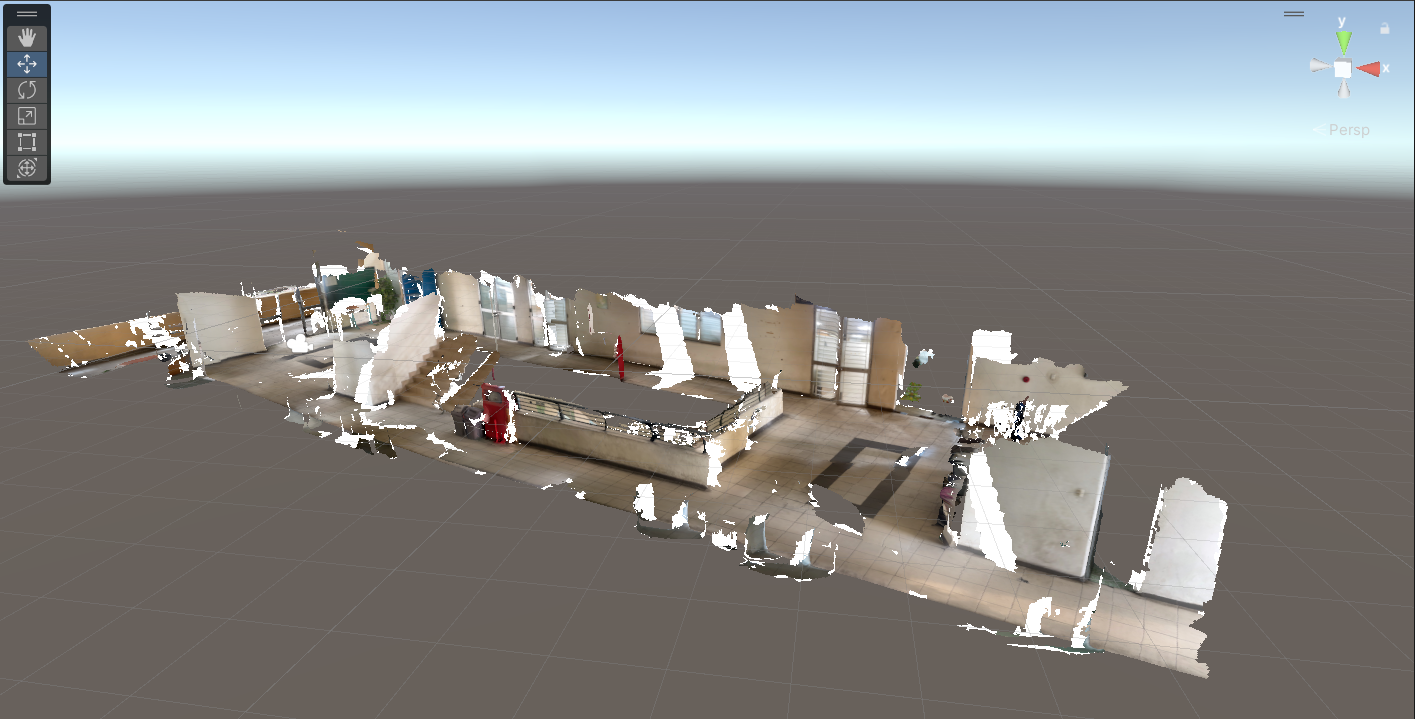
\includegraphics[scale=0.3]{content/resources/images/chap-problems-solutions/construct-environment-4.PNG}
  \caption{A scan of the 8th floor of building I at HCMUS.}
  \label{fig:construct-environment-4}
\end{figure}

\subsubsection{Multiple Areas}
Since the scanning area is limited, we need to create multiple models and merge them for a larger space—specifically, the I building. Fortunately, the Vuforia Creator application supports capturing adjacent areas. Once we have the 3D model of an area, we can continue scanning the neighboring area by selecting \textit{Capture Aligned Area}. After that, we must re-scan approximately $25\%$ of the current area that overlaps with the adjacent area so that the application can automatically scale it. This process can be repeated until the entire spacious area is fully scanned. All the separate scanned models will be automatically scaled and correctly aligned with each other once imported into the Unity project as Area Targets. Figure~\ref{fig:construct-environment-5} shows the 7th and 8th floors of the I building at HCMUS, constructed by three separate scans.

\begin{figure}[ht]
  \centering
  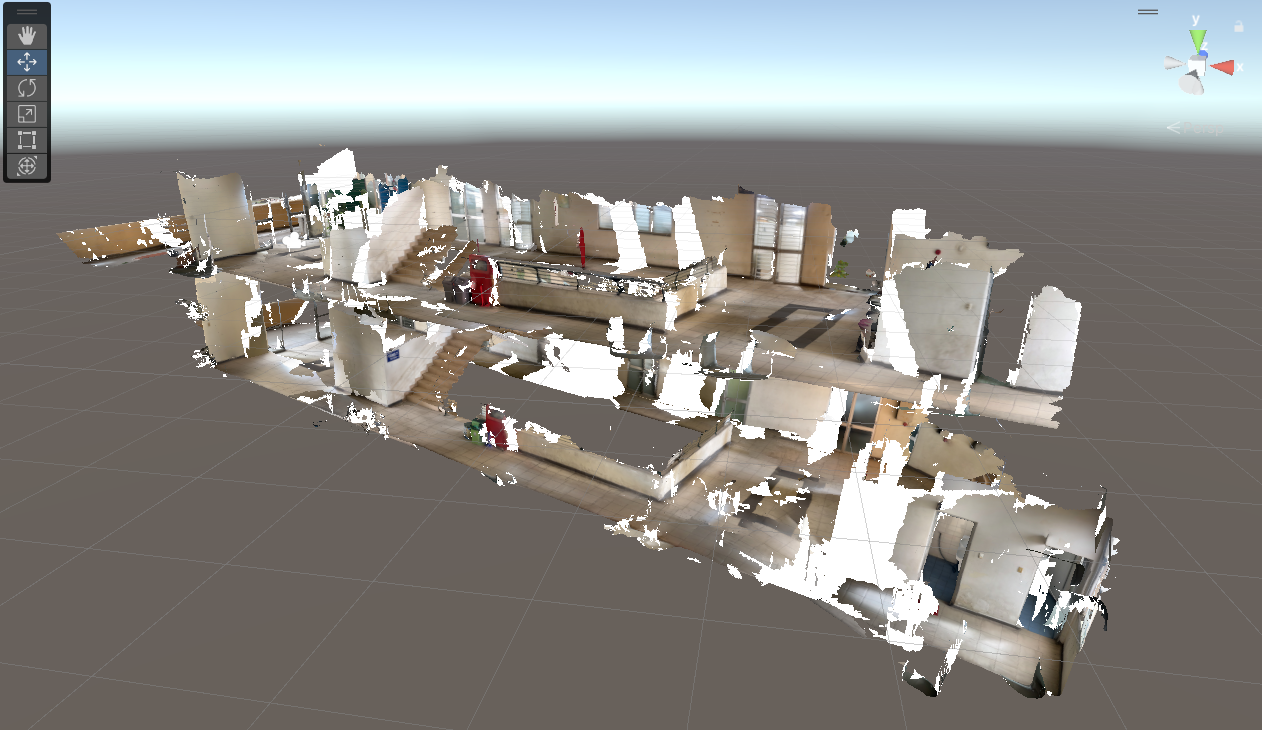
\includegraphics[scale=0.3]{content/resources/images/chap-problems-solutions/construct-environment-5.PNG}
  \caption{Combination of scans from the 7th and 8th floors of building I at HCMUS.}
  \label{fig:construct-environment-5}
\end{figure}

\begin{figure}[ht]
  \centering
  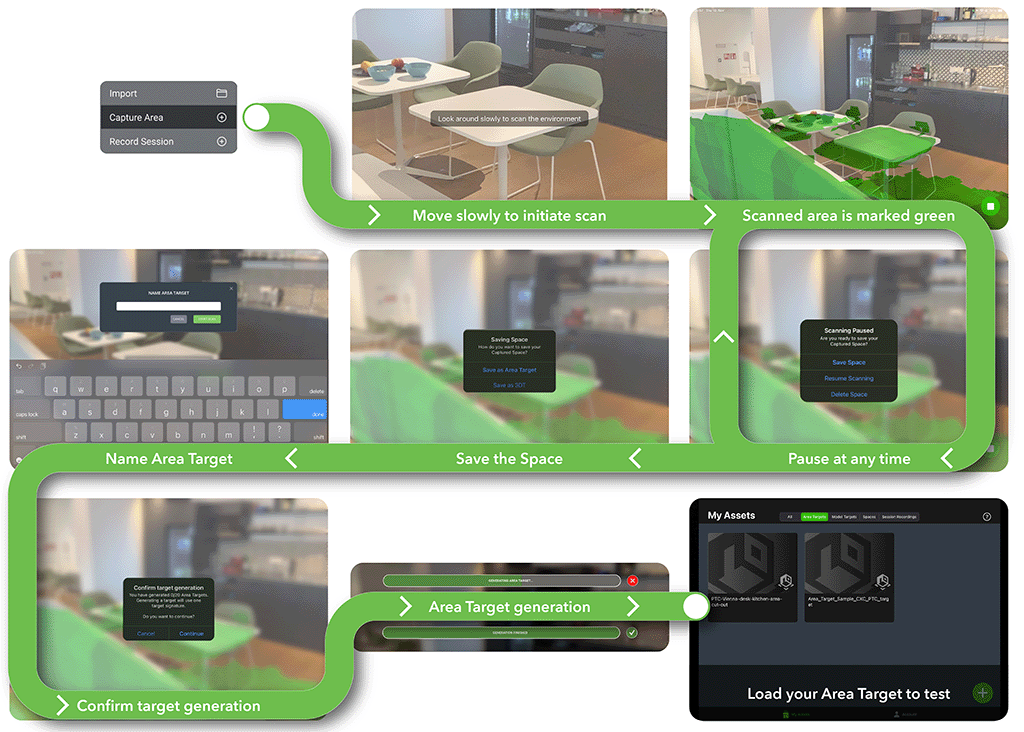
\includegraphics[scale=1]{content/resources/images/chap-problems-solutions/construct-environment-6.PNG}
  \caption{The workflow of generating a scan. \\ \small{Source: \url{https://developer.vuforia.com/library/tools/creator-app}}}
  \label{fig:construct-environment-6}
\end{figure}

\section{Environment Tracking Through Mobile's Camera}
\subsection{Problem Statement}
For the AR application to display navigation labels or arrows, it must correctly detect the environment through the mobile's camera to locate the user's position with respect to the predefined environment, which serves as the basis for placing navigation objects. In addition, changes in positions and angles must also be tracked to ensure that the objects are rendered accurately.

\subsection{Solution}

\subsubsection{Area Targets}
Vuforia Engine provides Area Targets, a powerful environment tracking feature. In Unity, a scanned 3D model of the target environment can be imported as an object of type Area Target, as shown in Figure~\ref{fig:construct-environment-4}. 

After obtaining the scanned 3D model, we import it into Unity as an Area Target. The default Main Camera is then replaced with the Vuforia ARCamera, and we must ensure that Device Tracking is enabled so the system can reliably establish the user’s pose relative to the scanned environment. The imported Area Target appears as a GameObject that includes a preview mesh—this mesh represents the physical space. It serves as the foundation for positioning the navigational labels or arrows. As discussed in Section~\ref{sec:construct-environment}, multiple Area Targets, if appropriately aligned during scanning, can be imported. They will appear at the correct positions relative to each other.

We enable runtime occlusion to improve realism by adding a runtime mesh representation. This process generates a dynamic mesh from the scanned data that acts as an occlusion layer. With the runtime mesh active, virtual objects will be appropriately hidden by physical obstacles (such as walls or furniture), ensuring that the AR content appears naturally embedded in the environment.

\subsubsection{Area Target Observer}\label{subsub:AreaTargetObserver}
Associated with Area Targets is the Area Target Observer, the component that actively manages the tracking of the imported 3D scan. It continuously monitors the pose and status of the Area Target within the scene, providing real-time updates to ensure that navigational labels or arrows remain accurately aligned with the physical environment. The observer retrieves key information—such as the target's bounding box, dimensions, and current tracking state (as shown in Figure~\ref{fig:environment-tracking-1})—which can be used to adjust the placement and orientation of augmented content dynamically.

\begin{figure}[ht]
  \centering
  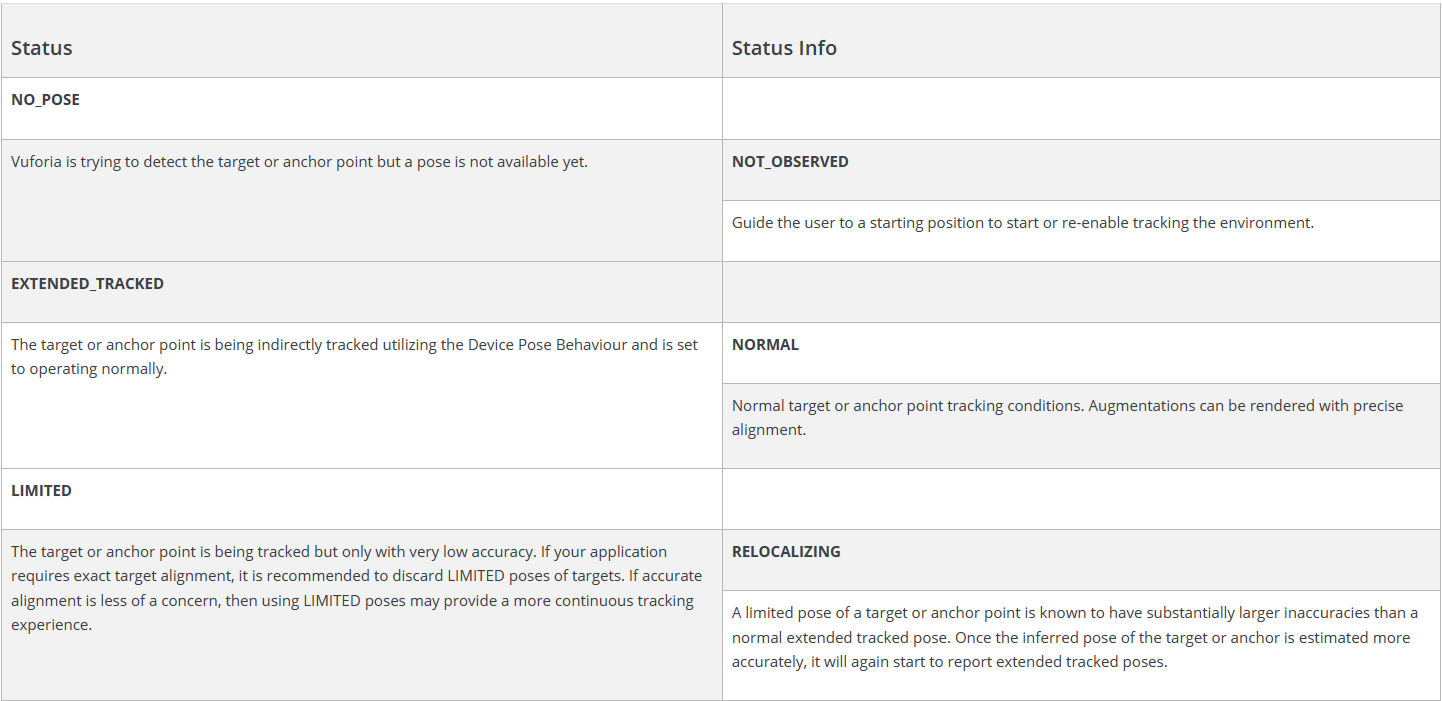
\includegraphics[scale=0.5]{content/resources/images/chap-problems-solutions/environment-tracking-1.PNG}
  \caption{The table listing the available pose status values for Area Targets. \\ \small{Source: \url{https://developer.vuforia.com/library/getting-started/pose-status-and-status-info-unity}}}
  \label{fig:environment-tracking-1}
\end{figure}

Beyond mere tracking, the observer facilitates a richer interaction experience by providing detailed feedback about the environmental context. It continuously assesses the tracking data's reliability, including various states indicating whether a target is fully tracked, partially tracked, or has lost tracking entirely. This detailed status information allows developers to fine-tune the augmented content’s behavior—adjusting its position, orientation, or scale—to adapt to environmental changes and maintain user immersion.

The tracking states of the Area Targets are reported and can be monitored through their Observer Behaviours. The \texttt{ObserverBehaviour} component associated with each Area Target can be retrieved as follows. Note that the Observer can only be retrieved for each Area Target, and it can only be accessed from within the Area Target object.

\begin{lstlisting}[style=cSharp]
ObserverBehaviour mObserverBehaviour = GetComponent<ObserverBehaviour>();
\end{lstlisting}

The current tracking status can be retrieved as follows.

\begin{lstlisting}[style=cSharp]
mObserverBehaviour.OnTargetStatusChanged += OnStatusChanged;
void OnStatusChanged(ObserverBehaviour behaviour, TargetStatus status)
{
    Debug.LogFormat("TargetName: {0}, Status is: {1}, StatusInfo is: {2}", behaviour.TargetName, status.Status, status.StatusInfo);
}
\end{lstlisting}

To further streamline the integration between tracking data and user interface feedback, the system employs global state variables managed through ScriptableObjects. A boolean variable is established for every Area Target to signify whether that particular area is currently being tracked.

\begin{lstlisting}[style=cSharp]
[CreateAssetMenu(fileName = "NewBoolVariable", menuName = "Variables/BoolVariable")]
public class BoolVariable : ScriptableObject
{
    public bool Value;
}
\end{lstlisting}

Whenever there is a change in the tracking status, we update the variables accordingly.

\begin{lstlisting}[style=cSharp]
public BoolVariable isTracked;
void OnStatusChanged(ObserverBehaviour behaviour, TargetStatus status)
{
    if (status.StatusInfo == StatusInfo.NORMAL)
    {
        isTracked.Value = true;
    }
    else
    {
        isTracked.Value = false;
    }
}
\end{lstlisting}

Collecting tracking status data from all monitored areas allows us to create a comprehensive overview of the environment, which is then used to display a clear and informative message to the user regarding their current floor. By aggregating this data, the system determines which specific floor the user is on and updates the interface with a message that confirms this location. This not only reinforces the user’s spatial awareness but also enhances the overall experience by keeping them informed in real time. In cases where none of the defined areas are actively being tracked, the system takes a proactive approach: it issues a warning to the user, advising them to either move towards a known area where tracking is reliable or to re-scan the QR code placed at pre-determined positions throughout the space. This re-scan prompt is designed to quickly recalibrate the tracking system and restore accurate positioning, ensuring users can seamlessly continue their navigation or interaction with the augmented reality content.

\begin{lstlisting}[style=cSharp]
public Text message;
public BoolVariable IsAreaTarget7;
public BoolVariable IsAreaTarget8;
void Update()
{
    if (IsAreaTarget7.Value) {
        message.text = "Tracking 7th floor.";
    }
    else if (IsAreaTarget8.Value) {
        message.text = "Tracking 8th floor.";
    }
    else {
        message.text = "No area target detected. Please move to the area target or re-scan for a position.";
    }
}
\end{lstlisting}

\begin{figure}[ht]
  \centering
  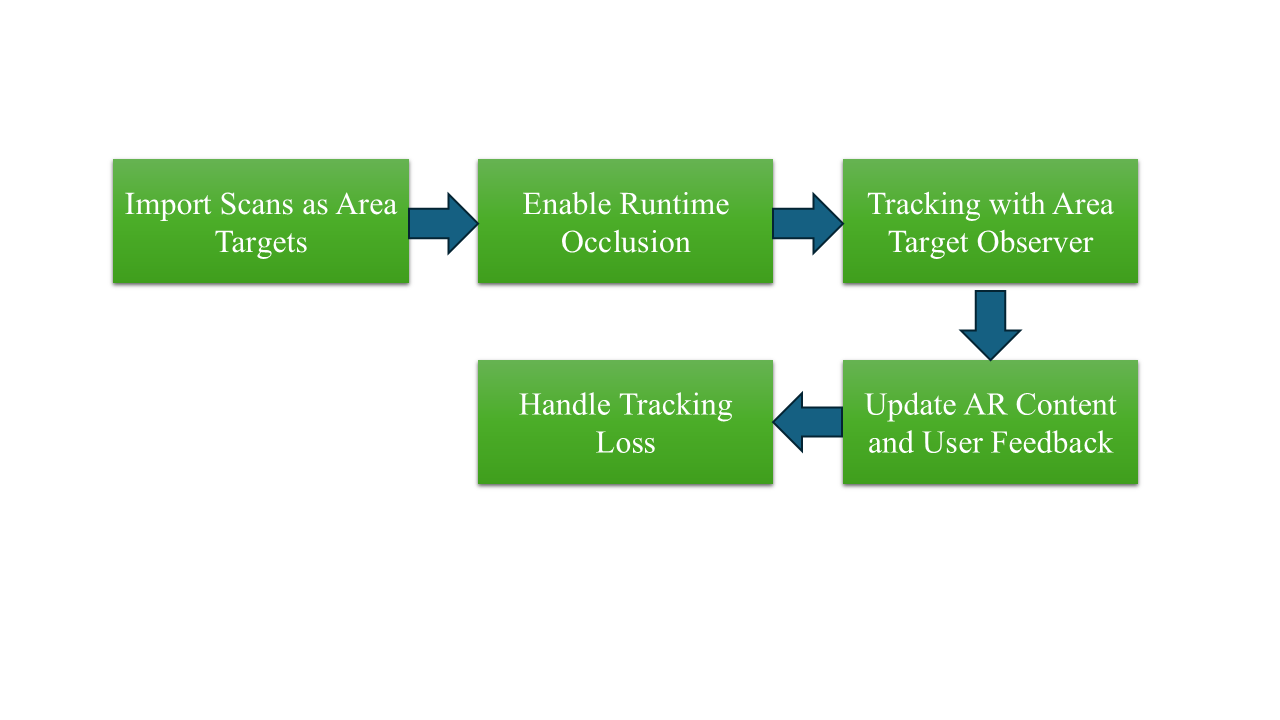
\includegraphics[scale=0.5]{content/resources/images/chap-problems-solutions/environment-tracking-0.PNG}
  \caption{Workflow of Environment Tracking with Area Targets}
  \label{fig:environment-tracking-0}
\end{figure}

\section{Indoor Positioning}
\subsection{Problem Statement}
Determining the user's precise starting position within an indoor environment is a critical first step for navigation. Unlike outdoor environments where GPS signals can be used reliably, indoor spaces lack such direct localization references. In expansive areas—where architectural features may be repetitive or ambiguous—automated recognition methods alone can struggle to identify the user's location uniquely. This challenge is compounded by the absence of distinct visual markers typically available in smaller, more controlled spaces.

\subsection{Solution}
\subsubsection{Auto Tracking for Small Area Targets}
For relatively small Area Targets, the positioning process can be fully automated. In these cases, the AR camera is designed to detect environmental features in real time and align them with the corresponding model data. This automatic alignment enables the system to accurately indicate the user's current position without requiring manual intervention.

As discussed in Section~\ref{subsub:AreaTargetObserver}, the tracking status is continuously monitored and updated. This information is then used to provide real-time feedback to the user, ensuring that necessary adjustments—such as reorienting the device or repositioning it slightly—can be made promptly to maintain optimal tracking performance.

Moreover, this automated approach simplifies the user experience in well-defined and controlled spaces. Since small Area Targets typically offer distinct and easily recognizable visual cues, the system can quickly and efficiently lock onto these features, resulting in a more stable and reliable positioning solution. However, it is essential to note that while auto-tracking is highly effective for small Area Targets, it may become less reliable when dealing with larger or multiple Area Targets, where environmental similarities (such as similar-looking floors) can cause ambiguities in target detection.

\subsubsection{Location Prior for Large Area Targets}\label{subsub:LocationPrior}
In environments featuring large or architecturally repetitive Area Targets, incorporating a location prior greatly enhances the localization process. A location prior provides direct guidance to the Area Target Observer, ensuring that targets are accurately aligned with their surrounding environment and improving the speed of the initial localization.

Location priors work by managing the loading of data from a set of activated Area Targets that have \texttt{requireExternalPositions} set to \texttt{VU\_TRUE}. The Vuforia Engine leverages this configuration to select and load the most relevant Area Targets based on both proximity and overlapping regions with the externally provided position. As a result, only the necessary target data is asynchronously loaded when an external position is set, which not only accelerates first-time localization but also minimizes tracking errors—particularly when the tracked position falls outside the intended region of an Area Target.

As a best practice, assigning an external prior for each large Area Target allows the Vuforia Engine to consistently choose the most appropriate and nearest targets among those activated. This is especially beneficial in scenarios where similar or repetitive features exist—such as different floors of the same building—ensuring a more reliable and efficient tracking experience.

\subsubsection{Positioning with QR Codes}
We implement a positioning system using QR Codes to provide accurate location tracking within a building. Predefined QR Codes are placed at pivotal positions, such as landings at the start of each new floor, to serve as location references. When users enter a floor or need to reposition after losing track of their environment, they can scan these QR Codes. The application will use the encoded position information as the location prior (as discussed in Section~\ref{subsub:LocationPrior}) to enhance relative positioning and tracking accuracy.

\subsubsubsection*{Generating QR Codes}
To encode positional data (x, y, z) into QR codes, we use Python's \texttt{qrcode} library. The following script generates a QR code containing JSON-formatted positional data:

\begin{lstlisting}[language=cSharp]
data = {"x": 1, "y": 2, "z": 3}
json_data = json.dumps(data)
qr = qrcode.QRCode(
    version=1,
    error_correction=qrcode.constants.ERROR_CORRECT_L,
    box_size=10,
    border=4,
)
qr.add_data(json_data)
qr.make(fit=True)

img = qr.make_image(fill='black', back_color='white')
img.save("qr_code.png")
\end{lstlisting}

This script generates a QR code containing the JSON-encoded coordinates of a location in the building.

\subsubsubsection*{Scanning QR Codes in Unity}
In Unity, we created a new scene that allows users to scan QR codes and extract encoded positional data. The scanning functionality is implemented using the \texttt{ZXing} library for barcode detection. Below are the key code segments and their detailed explanations.

\begin{itemize}
    \item \textbf{Defining the QRData Class}

    \begin{lstlisting}[style=cSharp]
    [Serializable]
    public class QRData
    {
        public int x;
        public int y;
        public int z;
    }
    \end{lstlisting}
    The \texttt{QRData} class is used to store positional data (x, y, z) extracted from the scanned QR code.

    \item \textbf{Variable Declarations and Camera Setup}
    \begin{lstlisting}[style=cSharp]
    [SerializeField] private RawImage _rawImageBackground;
    [SerializeField] private AspectRatioFitter _aspectRatioFitter;
    [SerializeField] private TextMeshProUGUI _textOut;
    [SerializeField] private RectTransform _scanZone;
    private bool _isCamAvailable;
    private WebCamTexture _cameraTexture;
    \end{lstlisting}
    These variables handle the camera feed and display the scanned QR code data on the UI.
    
    \begin{lstlisting}[style=cSharp]
    void Start()
        SetUpCamera();
    \end{lstlisting}
    When the scene starts, the \texttt{Start()} function calls \texttt{SetUpCamera()} to initialize the camera.

    \item \textbf{Setting Up the Camera for QR Scanning}
        \begin{lstlisting}[style=cSharp]
        private void SetUpCamera(){
            WebCamDevice[] devices = WebCamTexture.devices;
            if (devices.Length == 0){
                _isCamAvailable = false;
                return;
            }
            for (int i = 0; i < devices.Length; i++){
                if (!devices[i].isFrontFacing){
                    _cameraTexture = new WebCamTexture(devices[i].name, 
                        (int)_scanZone.rect.width, (int)_scanZone.rect.height);
                }
            }
            _cameraTexture.Play();
            _rawImageBackground.texture = _cameraTexture;
            _isCamAvailable = true;
        }
        \end{lstlisting}
        The \texttt{SetUpCamera()} function checks available camera devices, selects the back camera, and starts capturing video.

    \item \textbf{Updating the Camera Feed Display}
        \begin{lstlisting}[style=cSharp]
        private void UpdateCameraRender(){
            if (!_isCamAvailable){
                return;
            }
            float ratio = (float)_cameraTexture.width / (float)_cameraTexture.height;
            _aspectRatioFitter.aspectRatio = ratio;
            int orientation = -_cameraTexture.videoRotationAngle;
            _rawImageBackground.rectTransform.localEulerAngles = new Vector3(0, 0, orientation);
        }
        \end{lstlisting}
        This function adjusts the camera feed's aspect ratio and rotation to align with the screen display.

    \item \textbf{QR Code Scanning and Data Processing}
    \begin{lstlisting}[style=cSharp]
    public void OnClickScan()
        Scan();
    \end{lstlisting}
    The \texttt{OnClickScan()} function is triggered when the user presses the scan button.

    \begin{lstlisting}[style=cSharp]
    private void Scan(){
        try{
            IBarcodeReader barcodeReader = new BarcodeReader();
            Result result = barcodeReader.Decode(
                _cameraTexture.GetPixels32(), 
                _cameraTexture.width, 
                _cameraTexture.height
            );
    
            if (result != null){
                try{
                    QRData qrData = JsonUtility.FromJson<QRData>(result.Text);
                    _textOut.text = $"x: {qrData.x}, y: {qrData.y}, z: {qrData.z}";
                }
                catch{
                    _textOut.text = "INVALID QR CODE FORMAT";
                }
            }
            else{
                _textOut.text = "FAILED TO SCAN QRCODE";
            }
        }
        catch{
            _textOut.text = "FAILED IN TRY";
        }
    }
    \end{lstlisting}
    The \texttt{Scan()} function uses \texttt{ZXing} to decode the QR code from the camera feed. If a valid QR code is detected, it converts the JSON-formatted string into a \texttt{QRData} object and displays the extracted coordinates on the UI. An error message is shown if the QR code is invalid or scanning fails.

    \item \textbf{Summary}
        \begin{itemize}
            \item \textbf{Camera Setup}: Retrieves available devices, selects the back camera, and starts video capture.
            \item \textbf{Camera Feed Update}: Adjusts the display aspect ratio and orientation.
            \item \textbf{QR Code Scanning}: Reads the QR code, verifies the format, and displays the decoded data.
        \end{itemize}
\end{itemize}

\subsubsubsection*{Integration in the Application}
When a user scans a QR code, the application extracts the encoded coordinates and uses them as the new reference position. This functionality ensures accurate indoor navigation, improving tracking performance in augmented reality applications using Vuforia Engine. After scanning a QR code, the application automatically starts a new tracking session, ensuring precise localization within the defined model area. In addition, 

This implementation provides a robust and scalable approach to positioning using QR codes, combining Python for QR code generation and Unity with ZXing for QR code scanning and interpretation.

\begin{figure}[ht]
  \centering
  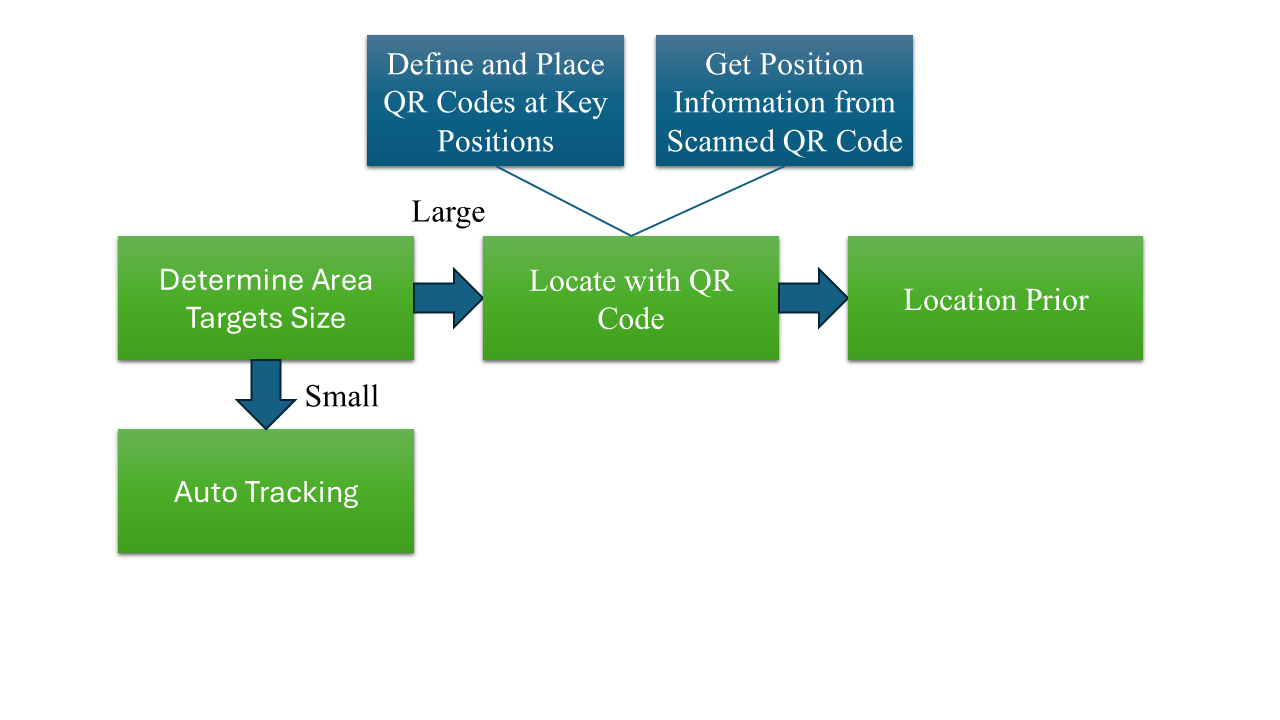
\includegraphics[scale=0.5]{content/resources/images/chap-problems-solutions/location-0.PNG}
  \caption{Workflow of Prior Location with QR Code}
  \label{fig:location-0}
\end{figure}
